\chapter*{\IfLanguageName{dutch}{Keuze software}{Software choice}}%
\label{ch:software}

Voor de implementatie van mijn microservices heb ik gekozen voor Istio, hoofdzakelijk omdat het een krachtig hulpmiddel is dat uitgebreide mogelijkheden biedt voor het beheren van microservices. Het levert een aantal functies die het beheer van microservices vereenvoudigen, zoals load balancing, service discovery, monitoring en tracing. Daarnaast biedt het ook een aantal geavanceerde functies, zoals circuit breaking, rate limiting en fault injection. Dit maakt het een zeer geschikt hulpmiddel voor het beheren van microservices in een productieomgeving ~\autocite{Istio}.

Om vertrouwd te raken met dit hulpmiddel, ben ik begonnen met het opzetten van een eenvoudige microservice die gebruikmaakt van voorbeeldgegevens.

De eerste stap was het downloaden van Istio. Dit kan worden gedaan door de volgende opdrachten uit te voeren:

\begin{lstlisting}[language=bash]
	$ curl -L https://istio.io/downloadIstio | sh -
	$ cd istio-1.21.1
	$ export PATH=$PWD/bin:$PATH
\end{lstlisting}

Nadat dit is voltooid, kan Istio worden geïnstalleerd met het volgende commando:

\begin{lstlisting}[language=bash]
	$ istioctl install --set profile=demo -y
\end{lstlisting}

Voordat u dit commando uitvoert, moet u echter eerst een Kubernetes-cluster hebben opgezet. Als u nog geen Kubernetes heeft geïnstalleerd, kunt u dit doen met het volgende commando:

\begin{lstlisting}[language=bash]
	$ brew install kubectl
\end{lstlisting}

Dit kan worden gedaan met behulp van Minikube en Hyperkit. De installatie van Minikube en Hyperkit kan worden uitgevoerd met de volgende commando's:

\begin{lstlisting}[language=bash]
	$ brew install minikube
	$ brew install hyperkit
\end{lstlisting}

Als Minikube en Hyperkit zijn geïnstalleerd, kunt u een cluster opzetten met het volgende commando:

\begin{lstlisting}[language=bash]
	$ minikube start --driver=hyperkit
\end{lstlisting}

Nadat u dit heeft gedaan, kunt u Istio installeren met het eerder genoemde commando. Als laatste stap moet u nog de Istio sidecar-injectie inschakelen met het commando:

\begin{lstlisting}[language=bash]
	$ kubectl label namespace default istio-injection=enabled
\end{lstlisting}

Vervolgens heb ik de voorbeeldapplicatie gedeployed met het volgende commando:

\begin{lstlisting}[language=bash]
	$ kubectl apply -f samples/bookinfo/platform/kube/bookinfo.yaml
\end{lstlisting}

Zorg ervoor dat alle pods en services actief zijn door de volgende commando's uit te voeren:

\begin{lstlisting}[language=bash]
	$ kubectl get services
	$ kubectl get pods
\end{lstlisting}

De volgende stap is het verbinden met een Istio gateway. Dit kan worden gedaan met het commando:

\begin{lstlisting}[language=bash]
	$ kubectl apply -f samples/bookinfo/networking/bookinfo-gateway.yaml
\end{lstlisting}

Dit kunt u controleren met het \verb|istioctl analyze| commando. Vervolgens moeten de ingress host en poort worden ingesteld. Dit heb ik gedaan door eerst het \verb|minikube tunnel| commando uit te voeren en vervolgens de volgende commando's uit te voeren:

\begin{lstlisting}[language=bash]
	$ export INGRESS_HOST=$(kubectl -n istio-system get service 
	istio-ingressgateway -o jsonpath='{.status.loadBalancer.ingress[0].ip}')
	$ export INGRESS_PORT=$(kubectl -n istio-system get service 
	istio-ingressgateway -o jsonpath='{.spec.ports[?(@.name=="http2")].port}')
	$ export SECURE_INGRESS_PORT=$(kubectl -n istio-system get service 
	istio-ingressgateway -o jsonpath='{.spec.ports[?(@.name=="https")].port}')
\end{lstlisting}

Om de gateway-URL te krijgen, kunt u het volgende commando uitvoeren:

\begin{lstlisting}[language=bash]
	$ export GATEWAY_URL=$INGRESS_HOST:$INGRESS_PORT
\end{lstlisting}

Nu kunt u de gateway-URL gebruiken om de applicatie te bekijken in uw browser. Met het volgende commando kunt u de weblink verkrijgen:

\begin{lstlisting}[language=bash]
	$ echo "http://$GATEWAY_URL/productpage"
\end{lstlisting}

Door dit commando uit te voeren, krijgt u de URL van de webpagina.

De volgende stap is om te zien wat er gebeurt op een dashboard. Dit kan worden bereikt met de volgende commando's:

\begin{lstlisting}[language=bash]
	$ kubectl apply -f samples/addons
	$ kubectl rollout status deployment/kiali -n istio-system
\end{lstlisting}

Vervolgens kunt u het Kiali-dashboard openen met het volgende commando:

\begin{lstlisting}[language=bash]
	$ istioctl dashboard kiali
\end{lstlisting}

Dit opent een dashboard waar u de interacties tussen de verschillende services kunt bekijken.

\begin{figure}[H]
	\centering	
	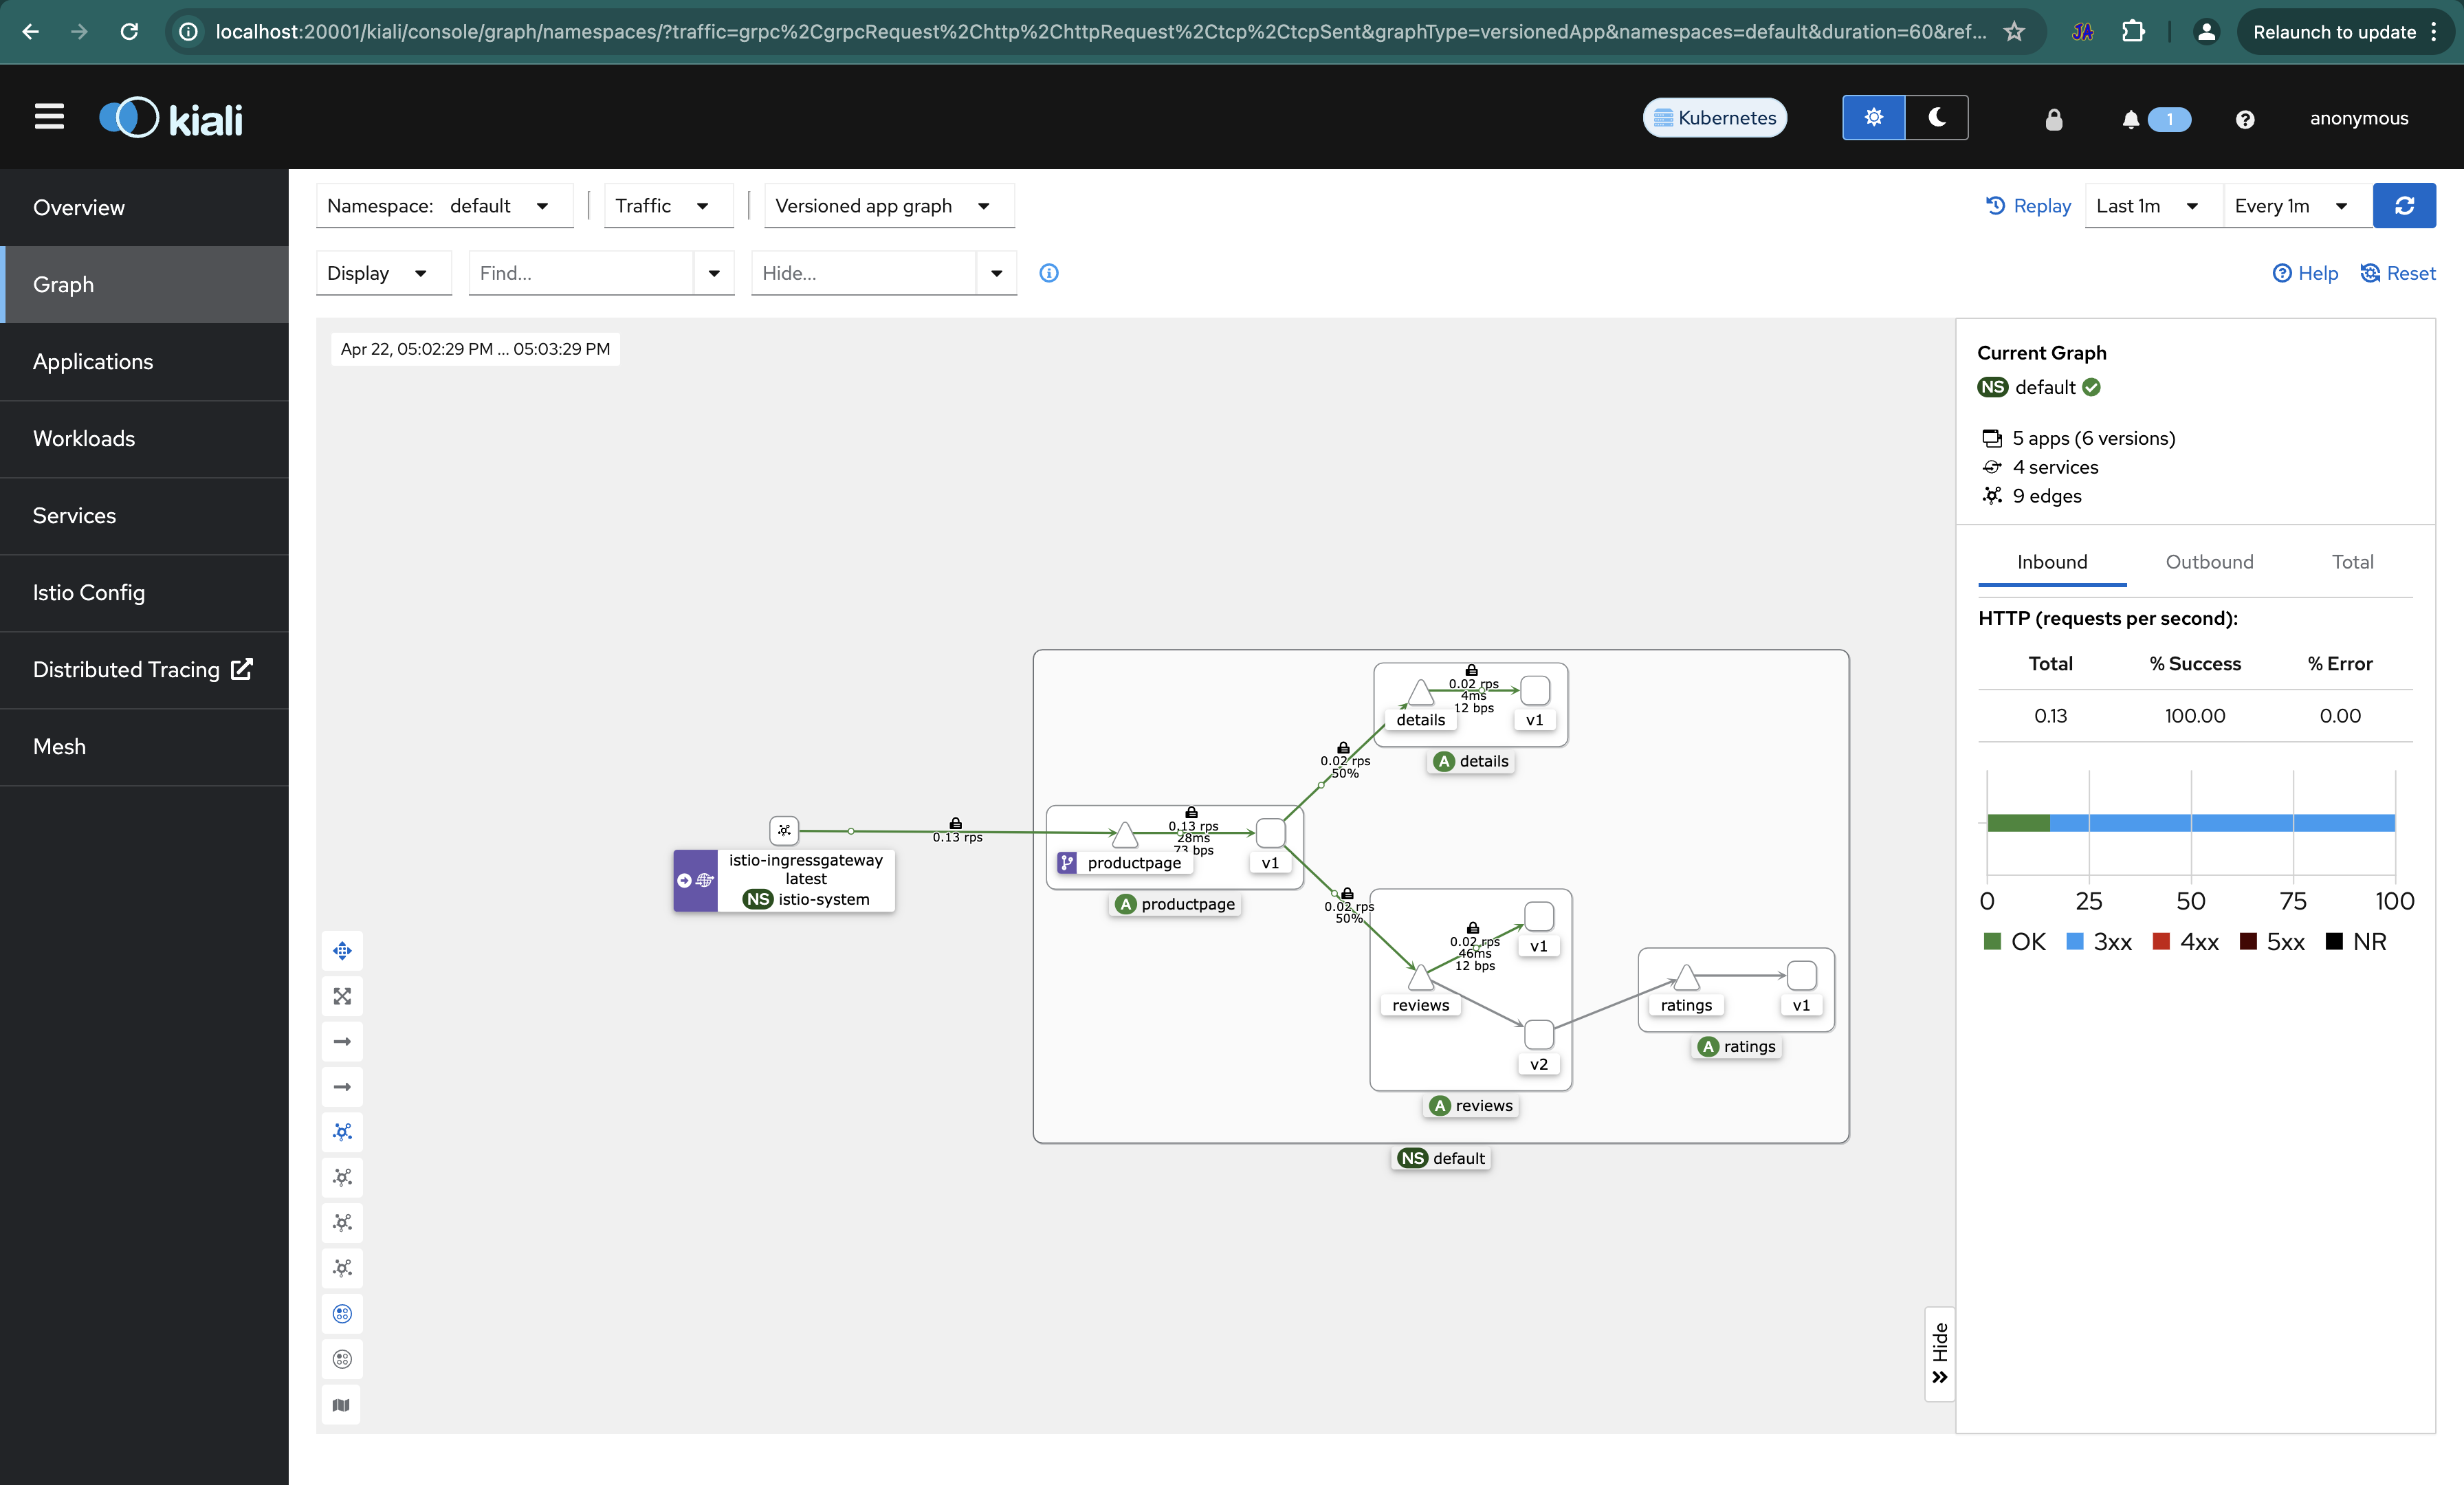
\includegraphics[width = \textwidth]{kailiConsole1.png} 
	\caption{Kaili Console} 
	\label{fig:kaili1} 
\end{figure}
\FloatBarrier
